\documentclass[12pt]{beamer}
\usetheme{default} 

\setbeamertemplate{navigation symbols}{} %gets rid of navigation symbols
\setbeamertemplate{footline}{} %gets rid of bottom navigation bars
\setbeamertemplate{footline}[page number]{} %use this for page numbers

\setbeamertemplate{footline}{%
  \raisebox{5pt}{\makebox[\paperwidth]{\hfill\makebox[10pt]{\scriptsize\insertframenumber~~}}}}

\setbeamertemplate{itemize items}[circle] %round bullet points
\setlength\parskip{10pt} % white space between paragraphs

\usepackage{wrapfig}
\usepackage{subfig}
\usepackage{setspace}
\usepackage{enumerate}
\usepackage{graphicx}
\usepackage{amsmath}
\usepackage{amsfonts}
\usepackage{amssymb}
\usepackage{amsthm}
\usepackage[UKenglish]{isodate}
\usepackage{tikz}
\usepackage{pgfplots}
\usepackage{natbib}
\usepackage{hyperref}
\hypersetup{
    colorlinks=true, 
    urlcolor=blue
}
\def\checkmark{\tikz\fill[scale=0.4](0,.35) -- (.25,0) -- (1,.7) -- (.25,.15) -- cycle;} 

% allow drawing arrows
\usetikzlibrary{arrows}
\tikzstyle{arrow}=[draw, -latex] 

% bracketing shortcuts
\newcommand{\paren}[1]{\left(#1\right)}
\newcommand{\sqbracket}[1]{\left[#1\right]}
\newcommand{\cbracket}[1]{\left\{#1\right\}}
\newcommand{\abs}[1]{\left\lvert#1\right\rvert}
\newcommand{\norm}[1]{\left\lVert#1\right\rVert}
% set up the argmin operator, argmax
\DeclareMathOperator*{\argmin}{arg\,min}
\DeclareMathOperator*{\argmax}{arg\,max}

\newcommand{\myframe}[1]{\begin{frame} \frametitle{#1}}

% New itemize environment, with spaces
\newenvironment{spaceitemize}
{ \begin{itemize}
    \setlength{\itemsep}{10pt}
    \setlength{\parskip}{0pt}
    \setlength{\parsep}{0pt}     }
{ \end{itemize}                  } 


% the preamble
\title{Day 3, Session 1: Installing R and RStudio}
\author{Jessica Williams-Nguyen and Brian D. Williamson}
\institute{EPI/BIOST Bootcamp 2017}
\date{26 September 2017}

% Start the document
\begin{document}
% The title page
\begin{frame}
\titlepage
\end{frame}

\myframe{
\includegraphics[width = 0.2\textwidth]{../Rlogo.png}}
R is a free software package that can be used for data analysis, graphics, and programming. 
\end{frame}

\myframe{Why R?}
R has many advantages, including:
\begin{spaceitemize}
\item Free!
\item Active group of contributors (anyone!)
\item Flexible
\end{spaceitemize}

However, this comes with some challenges:
\begin{spaceitemize}
\item Sometimes packages don't do what they say they do...
\begin{itemize}
\item ...but you can trust basically anything written by the R Core Team, the \href{https://www.rstudio.com/products/rpackages/}{RStudio Team}, \href{http://hadley.nz/}{Hadley Wickham}, or \href{https://github.com/yihui}{Yihui Xie}
\end{itemize}
\end{spaceitemize}
\end{frame}


\myframe{
\includegraphics[width = 0.2\textwidth]{../RStudiologo.png}}
\end{frame}

\myframe{Why RStudio?}

\end{frame}


\myframe{Why two programs?}
R is a programming software, prepackaged with a graphical user interface (GUI). However, R programs can be executed from the command line without an interactive interface.

RStudio is a GUI, and is a helpful tool for working in R. Using RStudio makes it easier to:
\begin{spaceitemize}
\item write R scripts to save your work, along with comments for what your code does
\item write reports with code embedded (using Rmarkdown)
\item organize your data analysis workflow (e.g., reading in data, access help files)
\end{spaceitemize}
\end{frame}

\myframe{Why two programs?}
At the end of the day: you are executing commands/programs in R, but using RStudio as an intuitive interface to the software (much like your operating system is a GUI to the machine language that your computer understands).
\end{frame}

\myframe{Installing R}
\begin{enumerate}
\item Go to \url{https://cran.r-project.org/}
\item[]
\item Choose the correct link under \textcolor{blue}{\underline{\texttt{Download and Install R}}}
\begin{spaceitemize}
\item Windows users, select \textcolor{blue}{\underline{\texttt{install R for the first time}}}
\item Mac users, click the \textcolor{blue}{\underline{\texttt{R-[replace with most recent version number].pkg}}} link and install
\item Linux users, I assume you know what you are doing
\end{spaceitemize}
\end{enumerate}

\end{frame}

\myframe{Installing RStudio}
\begin{enumerate}
\item Go to \url{https://www.rstudio.com/}
\item[]
\item Scroll down until you see the headers for \textcolor{blue}{\texttt{RStudio}}, \textcolor{blue}{\texttt{Shiny}}, and \textcolor{blue}{\texttt{R Packages}}  (see figure)
\item[]
\item Click \textcolor{blue}{\underline{Download}}
\item[] 
\item Click the green download button in the column for \texttt{RStudio Desktop}
\item[]
\item Choose the correct installer for your operating system and click the link
\end{enumerate}
\centering
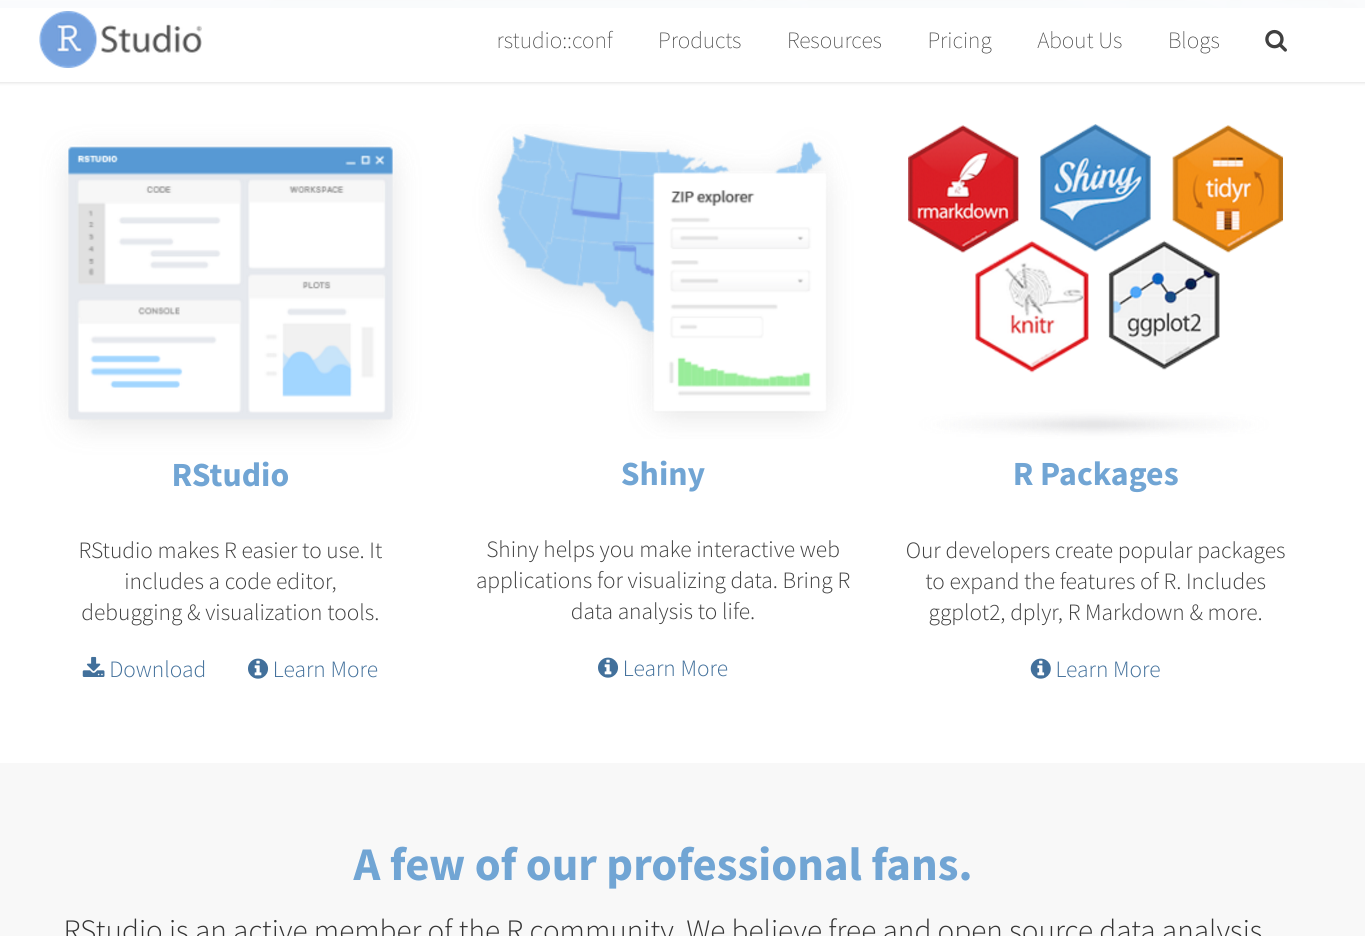
\includegraphics[width = 0.5\textwidth]{../rstudio_download.png}
\end{frame}

\myframe{R and Windows}

\end{frame}

\myframe{R and Mac/Linux}

\end{frame}

\end{document}